\lab{Convolution and Filtering}{Convolution and Filtering}
\objective{The Fourier transform reveals information in the frequency domain about signals and images that might not be apparent in the usual time (sound) or spatial (image) domain.
% It provides an extremely powerful tool to analyze difficult problems simply.
In this lab, we use the discrete Fourier transform to efficiently convolve sound signals and filter out some types of unwanted noise from both sounds and images.
This lab is a continuation of the Discrete Fourier Transform lab and should be completed in the same Jupyter Notebook.}

\section*{Convolution} % ======================================================

Mixing two sounds signals---a common procedure in signal processing and analysis---is usually done through a \emph{discrete convolution}.
% Recall that sound is modeled with discrete samples of a sound wave in rapid succession.
Given two periodic sound sample vectors $\f$ and $\g$ of length $n$, the discrete convolution of $\f$ and $\g$ is a vector of length $n$ where the $k$th component is given by
\begin{align}
(\f \ast \g)_k = \sum_{j=0}^{n-1} f_{k-j}g_j,\qquad k = 0,1,2,\dots,n-1.
\label{eq:naive-convolve}
\end{align}

Since audio needs to be sampled frequently to create smooth playback, a recording of a song can contain tens of millions of samples; even a one-minute signal has $2,646,000$ samples if it is recorded at the standard rate of $44,100$ samples per second ($44,100$ Hz).
The na\"ive method of using the sum in \eqref{eq:naive-convolve} $n$ times is $O(n^2)$, which is often too computationally expensive for convolutions of this size.

Fortunately, the discrete Fourier transform (DFT) can be used compute convolutions efficiently.
The \emph{finite convolution theorem} states that the Fourier transform of a convolution is the element-wise product of Fourier transforms:
\begin{align}
F_n(\f \ast \g) = n(F_n\f)\odot (F_n\g).
\label{eq:convolution-theorem}
\end{align}
In other words, convolution in the time domain is equivalent to component-wise multiplication in the frequency domain.
Here $F_n$ is the DFT on $\mathbb{R}^n$, $\ast$ is discrete convolution, and $\odot$ is component-wise multiplication. % (the \emph{Hadamard product}).
Thus, the convolution of $\f$ and $\g$ can be computed by
\begin{align}
\f \ast \g = nF_n^{-1}((F_n\f)\odot (F_n\g)),
\label{eq:fft-convolution}
\end{align}
where $F_n^{-1}$ is the \emph{inverse discrete Fourier transform} (IDFT).
The fast Fourier transform (FFT) puts the cost of \eqref{eq:fft-convolution} at $O(n\log{n})$, a huge improvement over the na\"ive method.

\begin{info} % Discard imaginaries after IDFT
Although individual samples are real numbers, results of the IDFT may have small complex components due to rounding errors.
These complex components can be safely discarded by taking only the real part of the output of the IDFT.

\begin{lstlisting}
>>> import numpy
>>> from scipy.fftpack import fft, ifft # Fast DFT and IDFT functions.

>>> f = np.random.random(2048)
>>> f_dft_idft = ifft(fft(f)).real      # Keep only the real part.
>>> np.allclose(f, f_dft_idft)          # Check that IDFT(DFT(f)) = f.
<<True>>
\end{lstlisting}
\end{info}

\begin{warn} % SciPy conventions
SciPy uses a different convention to define the DFT and IDFT than this and the previous lab, resulting in a slightly different form of the convolution theorem.
Writing SciPy's DFT as $\hat{F}_n$ and its IDFT as $\hat{F}_n^{-1}$, we have $\hat{F}_n = n F_n$, so \eqref{eq:fft-convolution} becomes
\begin{align}
\f \ast \g = \hat{F}_n^{-1}((\hat{F}_n\f)\odot (\hat{F}_n\g)),
\label{eq:fft-convolution-scipy}
\end{align}
without a factor of $n$.
Use \eqref{eq:fft-convolution-scipy}, not \eqref{eq:fft-convolution}, when using \li{fft()} and \li{ifft()} from \li{scipy.fftpack}.
\end{warn}

\subsection*{Circular Convolution} % ------------------------------------------

The definition \eqref{eq:naive-convolve} and the identity \eqref{eq:fft-convolution} require $\f$ and $\g$ to be periodic vectors.
However, the convolution $\f \ast \g$ can always be computed by simply treating each vector as periodic.
The convolution of two raw sample vectors is therefore called the \emph{periodic} or \emph{circular convolution}.
This strategy mixes sounds from the end of each signal with sounds at the beginning of each signal.

\begin{problem} % Circular convolution.
\item Implement the \li{__mul__()} magic method for the \li{SoundWave} class so that if \li{A} and \li{B} are \li{SoundWave} instances, \li{A * B} creates a new \li{SoundWave} object whose samples are the circular convolution of the samples from \li{A} and \li{B}.
If the samples from \li{A} and \li{B} are not the same length, append zeros to the shorter array to make them the same length before convolving.
Use \li{scipy.fftpack} and \eqref{eq:fft-convolution-scipy} to compute the convolution, and raise a \li{ValueError} if the sample rates from \li{A} and \li{B} are not equal.

A circular convolution creates an interesting effect on a signal when convolved with a segment of white noise: the sound loops seamlessly from the end back to the beginning.
To see this, generate two seconds of white noise (at the same sample rate as \texttt{tada.wav}) with the following code.
\begin{lstlisting}
>>> rate = 22050        # Create 2 seconds of white noise at a given rate.
>>> white_noise = np.random.randint(-32767, 32767, rate*2, dtype=np.int16)
\end{lstlisting}
Next, convolve \texttt{tada.wav} with the white noise.
Finally, use the \li{>>} operator to append the convolution result to itself.
This final signal sounds the same from beginning to end, even though it is the concatenation of two signals.
\end{problem}

\subsection*{Linear Convolution} % --------------------------------------------

Although circular convolutions can give interesting results, most common sound mixtures do not combine sounds at the beginning of one signal with sounds at the end of another.
Whereas circular convolution assumes that the samples represent a full period of a periodic function, \emph{linear convolution} aims to combine non-periodic discrete signals in a way that prevents the beginnings and endings from interacting.
Given two samples with lengths $n$ and $m$, the simplest way to achieve this is to pad both samples with zeros so that they each have length $n+m-1$, compute the convolution of these larger arrays, and take the first $n+m-1$ entries of that convolution.

\begin{problem} % Linear convolution.
\item Implement the \li{__pow__()} magic method for the \li{SoundWave} class so that if \li{A} and \li{B} are \li{SoundWave} instances, \li{A ** B} creates a new \li{SoundWave} object whose samples are the linear convolution of the samples from \li{A} and \li{B}.
Raise a \li{ValueError} if the sample rates from \li{A} and \li{B} are not equal.

Because \li{scipy.fftpack} performs best when the length of the inputs is a power of $2$, start by computing the smallest $2^a$ such that $2^a \ge n + m - 1$, where $a\in\mathbb{N}$ and $n$ and $m$ are the number of samples from \li{A} and \li{B}, respectively.
Append zeros to each sample so that they each have $2^a$ entries, then compute the convolution of these padded samples using \eqref{eq:fft-convolution-scipy}.
Use only the first $n + m - 1$ entries of this convolution as the samples of the returned \li{SoundWave} object.

To test your method, read \texttt{CGC.wav} and \texttt{GCG.wav}.
Time (separately) the convolution of these signals with \li{SoundWave.__pow__()} and with \li{scipy.signal.fftconvolve()}.
Compare the results by listening to the original and convolved signals.
\label{prob:fft-linear-convolution}
\end{problem}

\begin{problem} % Convolve the balloon pop with Chopin.
Clapping in a large room with an echo produces a sound that resonates in the room for up to several seconds.
This echoing sound is referred to as the \emph{impulse response} of the room, and is a way of approximating the acoustics of a room.
When the sound of a single instrument in a carpeted room is convolved with the impulse response from a concert hall, the new signal sounds as if the instrument is being played in the concert hall.

The file \texttt{chopin.wav} contains a short clip of a piano being played in a room with little or no echo, and \texttt{balloon.wav} is a recording of a balloon being popped in a room with a substantial echo (the impulse).
Use your method from Problem \ref{prob:fft-linear-convolution} or \li{scipy.signal.fftconvolve()} to compute the linear convolution of \texttt{chopin.wav} and \texttt{balloon.wav}.
% Listen to the new signal; there should be echo in the piano recording.
\end{problem}

\section*{Filtering Frequencies with the DFT} % ===============================

The DFT also provides a way to clean a signal by altering some of its frequencies.
Consider \texttt{noisy1.wav}, a noisy recording of a short voice clip.
The time-domain plot of the signal only shows that the signal has a lot of static.
On the other hand, the signal's DFT suggests that the static may be the result of some concentrated noise between about $1250$--$2600$ Hz.
Removing these frequencies could result in a much cleaner signal.

\begin{figure}[H]
\captionsetup[subfigure]{justification=centering}
\centering
\begin{subfigure}{.53\textwidth}
    \centering
    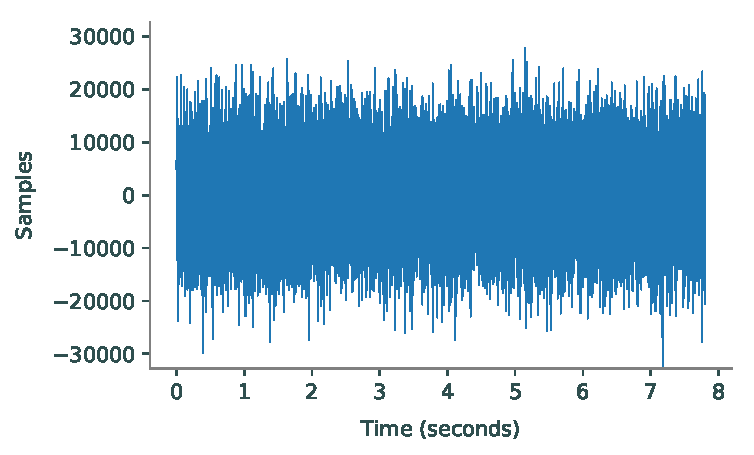
\includegraphics[width=\linewidth]{figures/noisy1.pdf}
\end{subfigure}%
\begin{subfigure}{.47\textwidth}
    \centering
    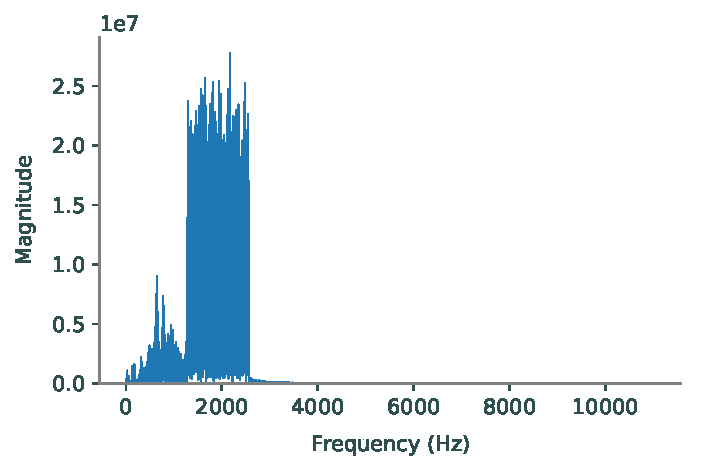
\includegraphics[width=\linewidth]{figures/noisy1_dft.pdf}
\end{subfigure}
\caption{The time-domain plot (left) and DFT (right) of \texttt{noisy1.wav}.}
\label{fig:fft-noisy-signal}
\end{figure}

To implement this idea, recall that the $k$th entry of the DFT array $\c = F_n \f$ corresponds to the frequency $v = k r / n$ in Hertz, where $r$ is the sample rate and $n$ is the number of samples.
Hence, the DFT entry $c_k$ corresponding to a given frequency $v$ in Hertz has index $k = v n / r$, rounded to an integer if needed.
In addition, since the DFT is symmetric, $c_{n-k}$ also corresponds to this frequency. %; any changes to $c_k$ must also be done to $c_{n-k}$ in order to alter the signal.
This suggests a strategy for filtering out an unwanted interval of frequencies $[v_\text{low},v_\text{high}]$ from a signal:
\begin{enumerate}
\item Compute the integer indices $k_\text{low}$ and $k_\text{high}$ corresponding to $v_\text{low}$ and $v_\text{high}$, respectively.
\item Set the entries of the signal's DFT from $k_\text{low}$ to $k_\text{high}$ and from $n-k_\text{high}$ to $n-k_{low}$ to zero, effectively removing those frequencies from the signal.
\item Take the IDFT of the modified DFT to obtain the cleaned signal.
\end{enumerate}
Using this strategy to filter \texttt{noisy1.wav} results in a much cleaner signal. %, shown in Figure \ref{fig:fft-noisy-cleaned}.
However, any ``good'' frequencies in the affected range are also removed, which may decrease the overall sound quality.
The goal, then, is to remove only as many frequencies as necessary.

\begin{figure}[H]
\captionsetup[subfigure]{justification=centering}
\centering
\begin{subfigure}{.53\textwidth}
    \centering
    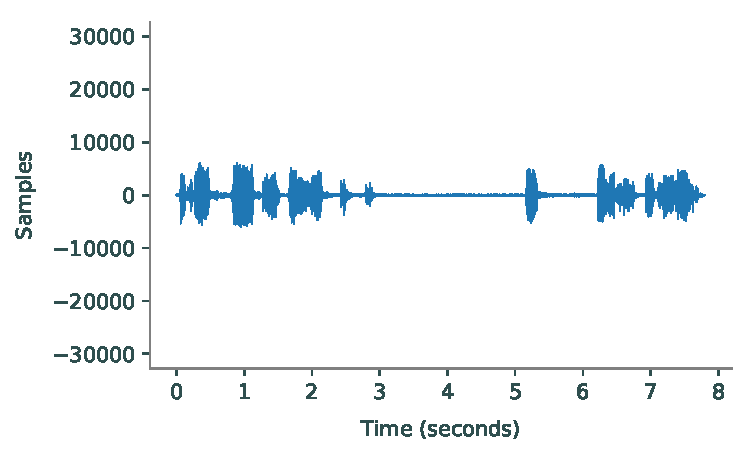
\includegraphics[width=\linewidth]{figures/noisy1_clean.pdf}
\end{subfigure}%
\begin{subfigure}{.47\textwidth}
    \centering
    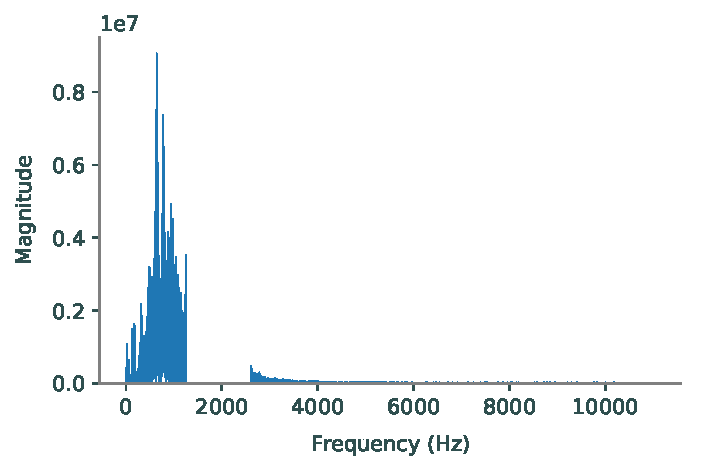
\includegraphics[width=\linewidth]{figures/noisy1_clean_dft.pdf}
\end{subfigure}
\caption{The time-domain plot (left) and DFT (right) of \texttt{noisy1.wav} after being cleaned.}
\label{fig:fft-noisy-cleaned}
\end{figure}

\begin{problem} % Clean up a noisy signal (The only thing we have to fear...)
\label{prob:fft-filter-frequencies}
Add a method to the \li{SoundWave} class that accepts two frequencies $v_\text{low}$ and $v_\text{high}$ in Hertz.
Compute the DFT of the stored samples and zero out the frequencies in the range $[v_\text{low}, v_\text{high}]$ (remember to account for the symmetry DFT).
Take the IDFT of the altered array and store it as the sample array.
% \\(Hint: be sure to sure the indices of the DFT array are integers.)

Test your method by cleaning \texttt{noisy1.wav}, then clean \texttt{noisy2.wav}, which also has some artificial noise that obscures the intended sound.
\\(Hint: plot the DFT of \texttt{noisy2.wav} to determine which frequencies to eliminate.)
\end{problem}

A digital audio signal made of a single sample vector with is called \emph{monoaural} or \emph{mono}.
When several sample vectors with the same sample rate and number of samples are combined into a matrix, the overall signal is called \emph{stereophonic} or \emph{stereo}.
This allows multiple speakers to each play one \emph{channel}---one of the original sample vectors---simultaneously.
``Stereo'' usually means there are two channels, but there may be any number of channels ($5.1$ surround sound, for instance, has five).

% \begin{warn}
Most stereo sounds are read as $n\times m$ matrices, where $n$ is the number of samples and $m$ is the number of channels (i.e., each column is a channel).
However, some functions, including Jupyter's embedding tool \li{IPython.display.Audio()}, receive stereo signals as $m\times n$ matrices (each row is a channel).
Be aware that both conventions are common.
% \end{warn}

% When a digital audio signal is played on a computer, the signal is sent to a speaker, which vibrates, producing sound waves.
% When multiple speakers are used, they can all produce the same signal or they can produce different signals.
% When there is only one signal, the sound is \emph{monoaural}, or \emph{mono}.  When speakers produce more than one signal, the overall signal is \emph{stereophonic}, or \emph{stereo}.
% Usually stereo means two, but there may be any number of signals ($5.1$ surround sound, for instance, has $5$).

% Most sounds are multi-dimensional, but can be treated similarly to mono sounds.
% The first and second columns of the array sample correspond to the signals for the left and right speaker respectively.

\begin{problem}
\label{prob:fft-vuvuzelas}
During the 2010 World Cup in South Africa, large plastic horns called vuvuzelas were blown excessively throughout the games.
Broadcasting organizations faced difficulties with their programs due to the incessant noise level.
Eventually, audio filtering techniques were used to cancel out the sound of the vuvuzela, which has a frequency of around $200$--$500$ Hz.

The file \li{vuvuzela.wav}\footnote{See \url{https://www.youtube.com/watch?v=g_0NoBKWCT8}.} is a stereo sound with two channels.
Use your function from Problem \ref{prob:fft-filter-frequencies} to clean the sound clip by filtering out the vuvuzela frequencies in each channel.
Recombine the two cleaned samples.
\end{problem}

% \begin{info} % Notch filtering and other filters
% The cleaning strategy of Problems \ref{prob:fft-filter-frequencies} and \ref{prob:fft-vuvuzelas} is called \emph{notch filtering} and is a special case of \emph{band-stop filtering}.
% \end{info}

\subsection*{The Two-dimensional Discrete Fourier Transform} % ----------------

The DFT can be easily extended to any number of dimensions.
Computationally, the problem reduces to performing the usual one-dimensional DFT iteratively along each of the dimensions.
For example, to compute the two-dimensional DFT of an $m \times n$ matrix, calculate the usual DFT of each of the $n$ columns, then take the DFT of each of the $m$ rows of the resulting matrix.
Calculating the two-dimensional IDFT is done in a similar fashion, but in reverse order: first calculate the IDFT of the rows, then the IDFT of the resulting columns.

\begin{lstlisting}
>>> from scipy.fftpack import fft2, ifft2

>>> A = np.random.random((10,10))
>>> A_dft = fft2(A)                 # Calculate the 2d DFT of A.
>>> A_dft_ifft = ifft2(A_dft).real  # Calculate the 2d IDFT.
>>> np.allclose(A, A_dft_ifft)
<<True>>
\end{lstlisting}

% The DFT for matrices is useful for a variety of image applications, including cleaning, compression, enhancement, and edge detection.
Just as the one-dimensional DFT can be used to remove noise in sounds, its two-dimensional counterpart can be used to remove ``noise'' in images.
The procedure is similar to the filtering technique in Problems \ref{prob:fft-filter-frequencies} and \ref{prob:fft-vuvuzelas}: take the two-dimensional DFT of the image matrix, modify certain entries of the DFT matrix to remove unwanted frequencies, then take the IDFT to get a cleaner version of the original image.
This strategy makes the fairly strong assumption that the noise in the image is periodic and corresponds to certain frequencies.
While this may seem like an unlikely scenario, it does actually occur in many digital images---for an example, try taking a picture of a computer screen with a digital camera.

\begin{figure}[H]
\captionsetup[subfigure]{justification=centering}
\centering
\begin{subfigure}{.4\textwidth}
    \centering
    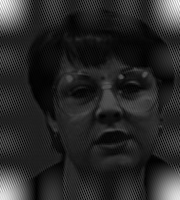
\includegraphics[width=\linewidth]{figures/blurry_face.png}
    \caption{The original blurry image.}
    \label{fig:blurry_face}
\end{subfigure}
\begin{subfigure}{.4\textwidth}
    \centering
    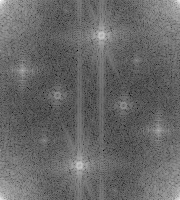
\includegraphics[width=\linewidth]{figures/blurry_fft.png}
    \caption{The DFT of the original image.}
    \label{fig:blurry_fft}
\end{subfigure}
\begin{subfigure}{.4\textwidth}
    \centering
    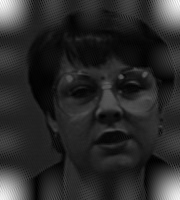
\includegraphics[width=\linewidth]{figures/improved_face.png}
    \caption{The improved image.}
    \label{fig:improved_face}
\end{subfigure}
\begin{subfigure}{.4\textwidth}
    \centering
    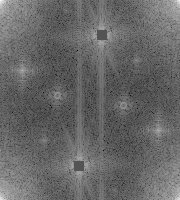
\includegraphics[width=\linewidth]{figures/covered_fft.png}
    \caption{The DFT of the improved image.}
    \label{fig:covered_fft}
\end{subfigure}
\caption{To remove noise from an image, take the DFT of the image and replace the abnormalities with values more consistent with the rest of the DFT.
Notice that the new image is less noisy, but only slightly.
This is because only some of the abnormalities in the DFT were changed; in order to further decrease the noise, we would need to further alter the DFT.}
\label{fig:image_fft}
\end{figure}

To begin cleaning an image with the DFT, take the two-dimensional DFT of the image matrix.
Identify \emph{spikes}---abnormally high frequency values that may be causing the noise---in the image DFT by plotting the log of the magnitudes of the Fourier coefficients.
With \li{cmap="gray"}, spikes show up as bright spots.
See Figures \ref{fig:blurry_face}--\ref{fig:blurry_fft}.

\begin{lstlisting}
# Read the image.
>>> import imageio
>>> im = imageio.read("noisy_face.png")

# Plot the log magnitude of the image's DFT.
>>> im_dft = fft2(image)
>>> plt.imshow(np.log(np.<<abs>>(im_dft)), cmap="gray")
>>> plt.show()
\end{lstlisting}

Instead of setting spike frequencies to zero (as was the case for sounds), replace them with values that are similar to those around them.
There are many ways to do this, but one convention is to simply ``patch'' each spike by setting portions of the DFT matrix to some set value, such as the mean of the DFT array.
See Figure \ref{fig:covered_fft}.

Once the spikes have been covered, take the IDFT of the modified DFT to get a (hopefully cleaner) image.
Notice that Figure \ref{fig:improved_face} still has noise present, but it is a slight improvement over the original.
However, it often suffices to remove some of the noise, even if it is not possible to remove it all with this method.

\begin{problem} % Clean an image.
The file \texttt{license\_plate.png} contains a noisy image of a license plate.
The bottom right corner of the plate has is a sticker with information about the month and year that the vehicle registration was renewed.
However, in its current state, the year is not clearly legible.

Use the two-dimensional DFT to clean up the image enough so that the year in the bottom right corner is legible.
This may require a little trial and error.
\end{problem}

\begin{comment}
\newpage
\section*{Additional Material} % ==============================================

\subsection*{Other Convolution Functions} % -----------------------------------

Talk about the options in \li{np.covolve()}, etc. (circular by default).
Use \li{scipy.ndimage.convolve()} to do circular convolution if needed (but the results must be shifted to match what we do).

\subsection*{Other Sound Filters} % -------------------------------------------

What we did is called a notch filter, blah blah blah...

\subsection{Other Image Filters} % --------------------------------------------

Overview of the following comment?

\end{comment}

\begin{comment} % VERY OLD (and bad) image filtering section ==================

\section*{Image Filters}

Recall that a computer stores an image as a 2-D array of pixel values (i.e., a matrix of intensities).
An image filter is a function that transforms an image by operating on it locally.
That is, to compute the $(ij)$th pixel value in the new image, an image filter uses only the pixels in a small neighborhood around the $(ij)$th pixel in the original image.

In this lab, we use a filter derived from the gradient of an image to find edges in an image.

\subsection*{Convolutions}

One example of an image filter is to \emph{convolve} an image with a filter matrix.
A filter matrix is a matrix whose height and width are relatively small odd numbers.
If the filter matrix is
\[
F = \begin{pmatrix}
f_{-1,-1}&f_{-1,0}&f_{-1,1}\\
f_{0,-1}&f_{0,0}&f_{0,1}\\
f_{1,-1}&f_{1,0}&f_{1,1}
\end{pmatrix},
\]
then the convolution of an image $A$ with $F$ is $A \ast F = (C_{ij})$ where
\begin{equation}\label{equ:convolve}
C_{ij} = \sum_{k=-1}^1 \sum_{\ell=-1}^1 f_{k\ell}A_{i+k,j+\ell}.
\end{equation}
Say $A$ is an $m \times n$ matrix. Here, we take $A_{ij}=0$ when $i \not \in \{1, \ldots m\}$ or $j \not \in \{1, \ldots, n\}$.
The value of $C_{ij}$ is a linear combination of the nearby pixel values, with coefficients given by $F$ (see Figure \ref{fig:convolution}).
In fact, $C_{ij}$ equals the Frobenius inner product of $F$ with the $3 \times 3$ submatrix of $A$ centered at $ij$.

\begin{figure}
\centering
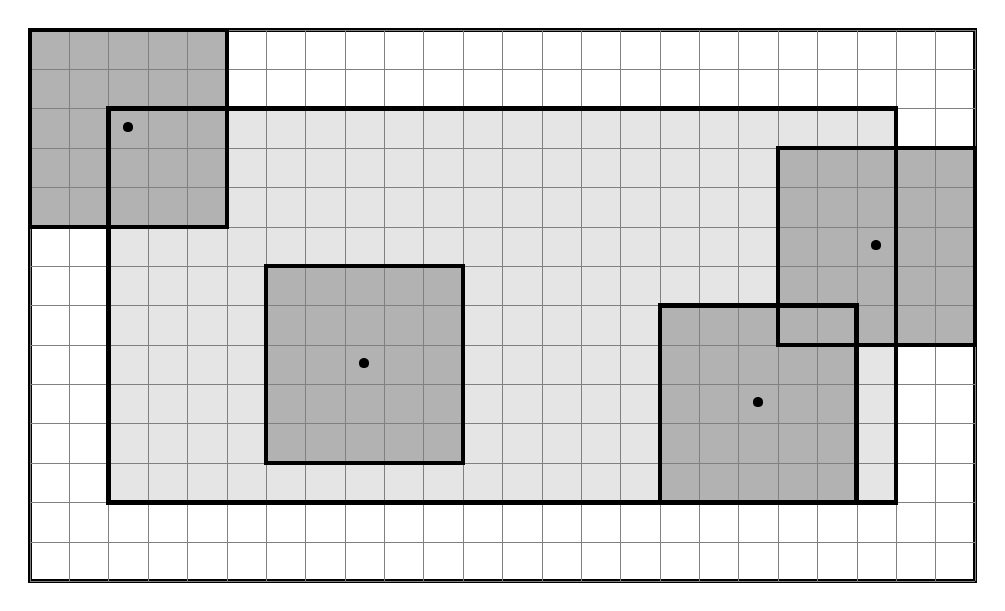
\begin{tikzpicture}
\node[draw, minimum width=12cm, minimum height=
    7cm, ultra thick](outer_rec)[]{};
\node[draw, minimum width=10cm, minimum height=
    5cm, ultra thick, fill=black!10!](inner_rec)[]{};
\node[draw, minimum width=2.5cm, minimum height=2.5cm,
    ultra thick, fill=black!30!](square1)at(-4.75,2.25){\textbullet};
\node[draw, minimum width=2.5cm, minimum height=2.5cm,
    ultra thick,fill=black!30!](square2)at(-1.75,-.75){\textbullet};
\node[draw, minimum width=2.5cm, minimum height=2.5cm,
    ultra thick, fill=black!30!](square3)at(4.75,.75){\textbullet};
\node[draw, minimum width=2.5cm, minimum height=2.5cm,
    ultra thick, fill=black!30!](square4)at(3.25,-1.25){\textbullet};
\draw[step=.5, ultra thin, color=black!50!](-6,-3.5)grid(6,3.5);

\node[draw, minimum width=10cm, minimum height=
    5cm, ultra thick, ][]{};
\node[draw, minimum width=2.5cm, minimum height=2.5cm,
    ultra thick]at(-4.75,2.25){};
\node[draw, minimum width=2.5cm, minimum height=2.5cm,
    ultra thick]at(-1.75,-.75){};
\node[draw, minimum width=2.5cm, minimum height=2.5cm,
    ultra thick]at(4.75,.75){};
\node[draw, minimum width=2.5cm, minimum height=2.5cm,
    ultra thick]at(3.25,-1.25){};
\end{tikzpicture}
\caption{This diagram illustrates how to convolve an image with a filter.
The light grey rectangle represents the original image $A$, and the dark grey squares are the filter $F$.
The larger rectangle is the image padded with zeros; i.e., all pixel values in the outer white band are 0.
To compute the entry of the convolution matrix $C$ located at a black dot, take the inner product of $F$ with the submatrix of the padded image centered at the dot.}
\label{fig:convolution}
\end{figure}

\subsubsection*{Implementation in NumPy}

Let us write a function that convolves an image with a filter.
You can test this function on the image \li{cameraman.jpg}, which appears in Figure \ref{fig:cameraman}.
The following code loads this image and plots it with matplotlib.

\begin{lstlisting}
>>> image = plt.imread('cameraman.jpg')
>>> plt.imshow(image, cmap = 'gray')
>>> plt.show()
\end{lstlisting}

Here is the function definition and some setup.

\begin{lstlisting}
1. def Filter(image, F):
2.     m, n = image.shape
3.     h, k = F.shape
\end{lstlisting}

To convolve \li{image} with the filter \li{F}, we must first \emph{pad} the array \li{image} with zeros around the edges.
This is because in \eqref{equ:convolve}, entries $A_{ij}$ are set to zero when $i$ or $j$ is out of bounds.
We do this by creating a larger array of zeros, and then making the interior part of the array equal to the original image (see Figure \ref{fig:convolution}).

For example, if the filter is a $3 \times 3$ matrix, then the following code pads the matrix with the appropriate number of zeros.

\begin{lstlisting}
 # Create a larger matrix of zeros
image_pad = np.zeros((m+2, n+2))
# Make the interior of image_pad equal to the original image
image_pad[1:1+m, 1:1+n] = image
\end{lstlisting}

We want to do this in general in our function.  Note that the number of zeros we need to pad our array depends on the size of the filter \li{F}.

\begin{lstlisting}
5.    image_pad = # Create an array of zeros of the appropriate size
6.   # Make the interior of image_pad equal to image
\end{lstlisting}

Finally, we iterate through the image to compute each entry of the convolution matrix.

\begin{lstlisting}
7.    C = np.zeros(image.shape)
8.    for i in range(m):
9.        for j in range(n):
10.            C[i,j] = # Compute C[i, j]
\end{lstlisting}

\subsubsection*{Gaussian Blur}

A \emph{Gaussian blur} is an image filter that operates on an image by convolving with the matrix
\[
G = \frac{1}{159}\begin{pmatrix}
2&4&5&4&2\\
4&9&12&9&4\\
5&12&15&12&5\\
4&9&12&9&4\\
2&4&5&4&2
\end{pmatrix}.
\]

Blurring an image can remove ``noise'', or random variation that is the visual analog of static in a radio signal (and equally undesirable).

\begin{problem}\label{prob:filter}
\leavevmode
Finish writing the function \li{Filter} by filling in lines 5, 6, and 10.  Hint: Note in \ref{equ:convolve}, $C_{ij}$ was calculated by summing from -1 to 1.  This is only the case if the filter \li{F} is $3 \times 3$. A slight modification is needed in the general case.  Test your function on the image \li{cameraman.jpg} using the Gaussian Blur. The result is in Figure \ref{fig:cameraman_blur}.
\end{problem}

\begin{figure}
\centering
\begin{subfigure}[b]{.49\textwidth}
\centering
% \includegraphics[width=\textwidth]{figures/cameraman.jpg}
\caption{Unfiltered image.}
\label{fig:cameraman}
\end{subfigure}
\begin{subfigure}[b]{.49\textwidth}
\centering
% \includegraphics[width=\textwidth]{figures/cameramanBlur.pdf}
\caption{Image after Gaussian blur is applied.}
\label{fig:cameraman_blur}
\end{subfigure}
\begin{subfigure}[b]{.49\textwidth}
\centering
% \includegraphics[width=\textwidth]{figures/edges.pdf}
\caption{Image after the Sobel filter is applied.}
\label{fig:cameraman_edges}
\end{subfigure}
\caption{Here is an example of a Gaussian blur and the Sobel filter applied to an image.
This photo, known as ``cameraman,'' is a standard test image in image processing.
A database of such images can be downloaded from \url{http://www.imageprocessingplace.com/root_files_V3/image_databases.htm}.}
\label{fig:cameraman1}
\end{figure}

\subsection*{Edge Detection}

Automatic detection of edges in an image can be used to segment or sharpen the image.
We find edges with the Sobel filter, which computes the gradient of the image at each pixel.
The magnitude of the gradient tells us the rate of change of the pixel values, and so large magnitudes should
correspond to edges within the image.
The Sobel filter is not a convolution, although it does use convolutions.

We can think of an image as a function from a $2 \times 2$ grid of points to $\mathbb{R}$.
The image maps a pixel location to an intensity.
It does not make sense to define the derivative of this function as a limit because the domain is discrete---a step size $h$ cannot take on arbitrarily small values.
Instead, we \emph{define} the derivative to be the centered difference quotient of the previous section.
That is, we define the derivative in the $x$-direction at the $ij$th pixel to be
\[
\frac{1}{2}A_{i+1, j} - \frac{1}{2}A_{i-1, j}.
\]

We can use a convolution to create a matrix $A_x$ whose $ij$th entry is the derivative of $A$ at the $ij$th entry, in the $x$-direction.
In fact, $A_x = A \ast S$, where
\[
S = \frac{1}{8}
\left[\begin{array}{ccc}
-1 & 0 & 1\\
-2 & 0 & 2\\
-1 & 0 & 1
\end{array}\right].
\]

Note that this convolution takes a weighted average of the $x$-derivatives at $(i, j)$, $(i, j+1)$, and $(i, j-1)$.
The derivative at $(i, j)$ is weighted by 2.
Using a weighted average instead of just the derivative at $(i, j)$ makes the derivative less affected by noise.

Now we can define the Sobel filter.
A Sobel filter applied to an image $A$ results in an array $B = (B_{ij})$ of 0's and 1's, where the 1's trace out the edges in the image.
By definition,
\[
B_{ij} = \left\{
     \begin{array}{ll}
       1 & \text{if}\; \;\|\nabla A(ij)\|_2 > M \\
       0 & \text{otherwise}.
     \end{array}
   \right.
\]
Here, $\nabla A(ij) = ((A \ast S)_{ij}, (A\ast S^T)_{ij})$ is the gradient of $A$ at the $ij$th pixel.
The constant $M$ should be ``sufficiently large'' enough to pick out those pixels with the largest gradient (i.e., those pixels that are part of an edge).
A good choice for $M$ is 4 times the average value of $\|\nabla A(ij)\|_2$ over the whole image $A$.

When the Sobel filter is applied to \li{cameraman.jpg}, we get the image in Figure \ref{fig:cameraman_edges}.
Here, the 1's in $B$ were mapped to ``white'' and the 0's were mapped to ``black.''

\begin{problem}
Write a function that accepts an image as input and applies the Sobel filter to the image.  Test your function on \li{cameraman.jpg}.  Hint: If you want to find the average of a matrix \li{A}, use the function \li{A.mean()}.
\end{problem}

\end{comment}
